\section{Introduction}
Pathfinding systems which operate on regular grids are commonly found in
academic literature; for example in application areas such as robotics 
\cite{choset05}, video games \cite{botea04,sturtevant05,bjornsson06} and 
planning \cite{thayer10,DBLP:conf/aips/HernandezMSK09,DBLP:conf/aips/WangB08,DBLP:conf/aips/BulitkoBLSS07}.
\par
In the context of single-agent pathfinding, and real-time video games in particular, 
it is often the case that queries sent to the pathfinding system  need to be solved as quickly as possible.
Traditionally, this requirement is met in one of two ways: (i) by reducing the size of the search space through hierarchical 
decomposition or (ii) through the development of improved heuristics to guide search.
In the case of hierarchical decomposition, techniques such as
HPA*~\cite{botea04} and PRA* ~\cite{sturtevant05} seek to construct and explore
a much reduced approximate state space.
These methods are fast and require no significant extra memory when compared to the classical
A* algorithm \cite{hart68}.
However, they have the disadvantage that solutions are not guaranteed to be optimal.
Meanwhile, in case of the improved heuristics, it has frequently been shown
that obtaining better informed results than the popular
Manhattan or Octile heuristic usually incurs significant memory overhead 
\cite{sturtevant09,goldberg05,Cazenave:06,bjornsson06}.
Furthermore, it is well known that even heuristics which differ from perfect information 
by at most a (small) additive constant, can still exhibit poor performance on a range of 
problems such as AI planning and graph search \cite{helmert08,pohl77}.
\par
Very recently a third class of methods, based on the idea of search space
reduction, has emerged as a promising alternative for speeding up pathfinding
search.
Algorithms of this type \cite{bjornsson06,pochter10,harabor10} are shown to produce 
results that are not only optimal but also memory efficient, particularly when compared 
with memory-based heuristics.
Additionally, they can significantly improve the performance of well known graph
search algorithms such as A*.
\par
In this paper we present Room-based Symmetry Reduction (RSR): a
symmetry-breaking search space reduction algorithm which recognises 
that there are often many paths of equal length between arbitrary pairs of tiles on a 
grid map.
The main idea then is to decompose the map in such a way that, 
given a particular pathfinding problem, it is possible to discard from consideration tiles which are on 
a symmetric path of equal length to the one ultimately returned as the solution.
RSR which uses an Empty Rectangular Rooms (ERR) decomposition, originally described in
\cite{harabor10}, to convert an arbitrary grid map into an equivalent grid map where only tiles from the 
perimeter of each empty room need to be explored during search (see Figure
\ref{fig-overview} for an overview).
%Though effective, the method is limited to 4-connected grid maps where only straight moves, and not diagonal, are
%allowed.
We extend that approach in several directions: (i) we generalise the method from 4-connected grid maps to 
the much more common 8-connected case and show how the higher branching factor associated 
with this domain makes effective symmetry elimination more challenging.
(ii) we develop a new offline pruning technique that reduces the number of nodes which
need to be explored during search.
(iii) we give a novel online pruning strategy which speeds up node expansion by selectively 
evaluating either all neighbours associated with a particular tile or only a small subset.
We show that in each case both optimality and completeness are preserved.
\par
We perform a thorough empirical analysis, comparing RSR with existing
symmetry-breaking algorithms~\cite{pochter10,harabor10}
on a number of synthetic and realistic benchmarks, including one well known set 
from the popular roleplaying game \emph{Baldur's Gate II}.
Our analysis allows us to identify distinct advantages over both benchmark algorithms.
Compared to Harabor and Botea's method \shortcite{harabor10}, 
we both extend the applicability and improve the speed
on the subset of instances where both methods are applicable.
Furthermore, we show that RSR and the swamp-based method of 
\citeauthor{pochter10}~\shortcite{pochter10}
have complementary strengths and identify classes of instances where
either RSR or swamps is more suitable.
We conclude that swamps are better suited for maps with
small open areas and their effectiveness reduces on maps with larger open areas.
In contrast, larger open areas allow RSR to build larger empty rooms and in such
cases there is a corresponding improvement in its search performance.


%TODO bring up to date and integrate in text
%On our test data the average performance of A* is increased by up to 9 times on 8-connected grid maps and up to
%18 times on 4-connected grid maps, depending on the topography of the map being used.


\begin{figure}[tb]
       \begin{center}
                       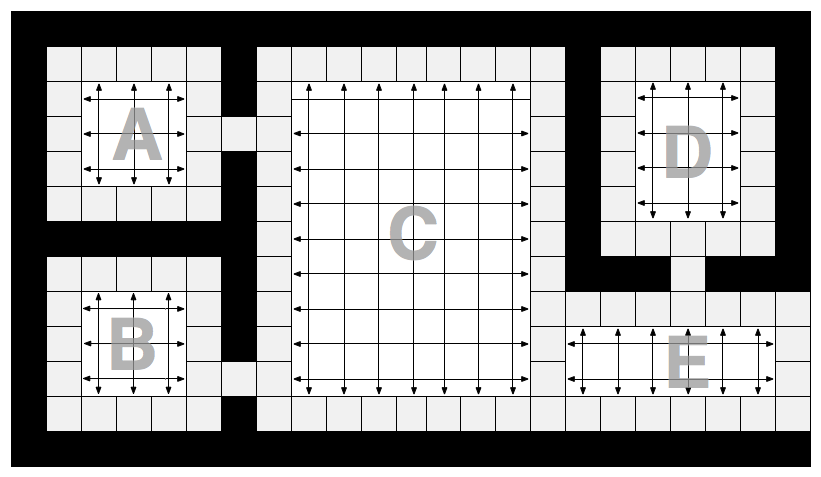
\includegraphics[scale=0.30, trim = 10mm 10mm 10mm 0mm]{diagrams/overview.png}
       \end{center}
	\vspace{-3pt}
       \caption{In \cite{harabor10} a 4-connected map is decomposed into a set of obstacle-free rooms from which are pruned all nodes except those on the perimeter.
				They are replaced with a small set of macro edges (arrows) that connect the perimeter nodes directly.}
       \label{fig-overview}
\end{figure}

